%% LaTeX2e class for student theses
%% appendix
%% 
%% Based on SDQ KIT Template by Erik Burger
%%
%% Karlsruhe Institute of Technology
%% Institute for Automation and Applied Informatics
%% AIDA Research Group
%%
%% Nicole Ludwig
%% nicole.ludwig@kit.edu
%%
%% Version 1.2, 2018-10-11


\iflanguage{english}
{\chapter{Appendix}}    % english style
{\chapter{Anhang}}      % german style
\label{chap:appendix}

\section{Model values}
\label{sec:appendix:Modelvalues}
\begin{table}[h]
    \centering
    \begin{tabular}{c|c|c}
         &  Start values & Identified values\\
         \hline
        $C_\text{inside}$& 407532 $J/W$ & 1109738 $J/W$\\
        $C_\text{envelope}$ & 24999045 $J/W$ & 24998602 $J/W$\\
        $C_\text{interior}$& 22960754 $J/W$ & 23859585 $J/W$\\
        $C_\text{floor}$ & 26118734 $J/W$ & 26079959 $J/W$\\
        $R_\text{inside}$ & 191 $K/W$ & 1.08710 $K/W$\\
        $R_\text{window}$ & 34 $K/W$ & 0.00251 $K/W$\\
        $R_\text{envelope}$ & 287 $K/W$ & 0,00008 $K/W$\\
        $R_\text{interior}$& 77 $K/W$ & 54602 $K/W$\\
        $R_\text{floor}$ & 749 $K/W$ & 2731 $K/W$\\
        $R_\text{in}$ & 191 $K/W$ & 191 $K/W$\\
        $f_\text{sol,inside}$ & 0,25 & 6.53161 $K/W$\\
        $f_\text{sol,envelope}$ &0,25 & -7.30656 $K/W$\\
    \end{tabular}
    \caption{Start and identified values of the model parameters}
    \label{tab:StartwerteSchätzung}
\end{table}

\section{Further training and verification diagrams}
\label{sec:appendix:Modelvalues}
\begin{figure}[h]
            \centering
            \includegraphics[width=14cm,height=5.5cm]{figure/Training.eps}
           \caption{Training of $T_\text{envelope}$ of the building model}
           \label{fig:trainingModelenvelope}
    \end{figure}
    \begin{figure}[h]
            \centering
            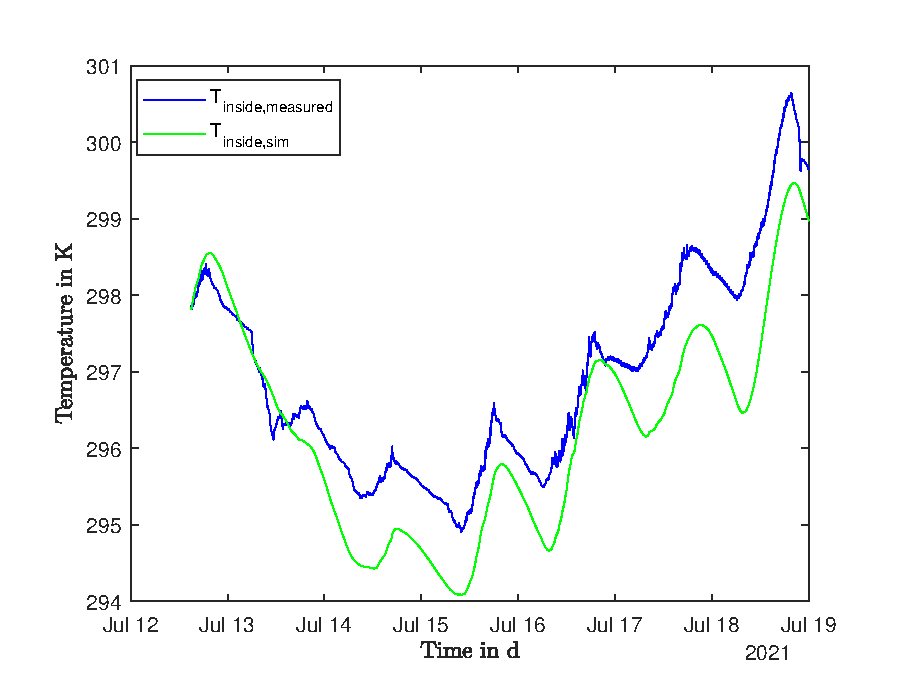
\includegraphics[width=7cm,height=5cm]{figure/Validation_inside.eps}
           \caption{Verification of $T_\text{envelope}$ of the building model}
           \label{fig:verificationModelenvelpe}
    \end{figure}
    
\section{Matrices of state-space formulation}
\label{sec:appendix:Matrizen}
    
    \begin{equation}
    B_1 = 
    \begin{pmatrix}
        1 & 0 \\
        0 & 0 \\
        0 & 0 \\
        0 & 0 \\
        -1 & 1 
    \end{pmatrix}
    \end{equation}
    \begin{equation}
	B_2
	\begin{pmatrix}
         f_{sun,inside} & 0 & \frac{1}{C_{inside}R_{window}} & 0\\
         0 & f_{sun,envelope} & \frac{1}{C_{envelope}R_{envelope}}&0\\
         0 & 0 & 0& 0\\
         0 & 0 & 0& 0\\
         0 & 0 & 0 & -1
    \end{pmatrix}
	\end{equation}
	\begin{equation}
	    C = 
	    \begin{pmatrix}
        1 & 0 & 0 & 0 & 0 \\
        \end{pmatrix}
	\end{equation}
	\begin{landscape}
	\begin{align} 
	A = \nonumber \\ 
	\begin{pmatrix}
    \frac{-1}{C_{inside}R_{inside}}-\frac{1}{C_{inside}R_{window}}-\frac{1}{C_{inside}R_{interior}}-\frac{1}{C_{inside}R_{floor}}   & \frac{1}{C_{inside}R_{inside}} & \frac{1}{C_{inside}R_{interior}} & \frac{1}{C_{inside}R_{floor}} & 0 \\
    \frac{1}{C_{envelope}R_{inside}}& \frac{-1}{C_{envelope}R_{envelope}}- \frac{1}{C_{envelope}R_{inside}} & 0 & 0 & 0 \\
    \frac{1}{C_{interior}R_{interior}} & 0 & -\frac{1}{C_{interior}R_{interior}} & 0 &0 \\
    \frac{1}{C_{floor}R_{floor}} & 0 & 0 & -\frac{1}{C_{floor}R_{floor}} &0 \\
    0 & 0 & 0 & 0 & 0
    \end{pmatrix} \nonumber\\ 
    \end{align}
    \end{landscape}

\section{Laboratory journal}
\label{sec:appendix:Laborbuch}
\textbf{Experiment: 16. July - 18. July 2021}
\begin{table}[H]
    \centering
    \begin{tabular}{c|c|c}
        \textbf{Time} & \textbf{Location} & \textbf{Incident }\\
        \hline
        \hline
        16.7.21 9.30pm & Room 1 & HoHe on\\
        & Room 2 & HoHeF on\\
        & Floor 2 & IH on\\
        && closed doors\\
        \hline
        18.7.21 0.00am & Room 2 & HoHeF off\\ 
        && rearrange HoHeF \\
        & Kitchen & HoHeF on\\
        \hline
        18.7.21 9.30pm & Room 1 & HoHe off\\
        & Kitchen & HoHeF off\\
        & Floor 2 & IH off\\
        && opened doors and windows\\
    \end{tabular}
    \caption{Laboratory journal: 16. July - 18. July 2021}
    \label{tab:Experiment1app}
\end{table}
\textbf{Experiment: 16. July - 18. July 2021}
\begin{table}[H]
    \centering
    \begin{tabular}{c|c|c}
        \textbf{Time} & \textbf{Location} & \textbf{Incident}\\
        \hline
        \hline
        26.7. - 27.7.21 & Kitchen & HoHeF on\\
        10.00pm - 5.00am & & closed door\\
        \hline
        27.7. - 28.7.21 & Kitchen & HoHeF on\\
        10.00pm - 4.00am & & closed door\\
        \hline
        28.7. - 29.7.21 & Kitchen & HoHeF on\\
        10.00pm - 5.00am & & opened door\\
        5.00am - 8.20am & & closed door\\
        \hline
        29.7. - 30.7.21 & all & breakdown PLC\\
        16.00pm - 9.30am & Kitchen & HoHeF still off\\
        \hline
        30.7.21 9.30pm & Room 1 & HoHe on\\
        & Room 2 & HoHeF on\\
        & Floor 2 & IH on\\
        && opened doors\\
        \hline
        31.7. - 1.8.21 & all & breakdown PLC\\
        2.30pm - 9.20am &&\\
        \hline
        31.7.21 4.00pm & Room 1 & HoHe off\\
        & Room 2 & HoHeF off\\
        7.30pm & Floor 2 & IH off\\
         & Room 2 & rearrange HoHeF \\
        \hline
        1.8.21 9.30pm & Room 1 & HoHe on\\
        & Kitchen & HoHeF on\\
       && PLC works\\
       \hline
        1.8.21 & all & breakdown PLC\\
        11.30am - 0.20pm &&\\
        \hline
        1.8.21 9.30pm & Room 1 & HoHe off\\
        & Kitchen & HoHeF off\\
        & Floor 2 & IH off\\
        && opened doors and windows\\
    \end{tabular}
    \caption{Laboratory journal: 26. July - 1. August 2021}
    \label{tab:Experiment2app}
\end{table}

\setcounter{figure}{0}
\section{Average comfort and grid services}
\label{sec:Average comfort and grid services}
\begin{figure}[H]
            \centering
            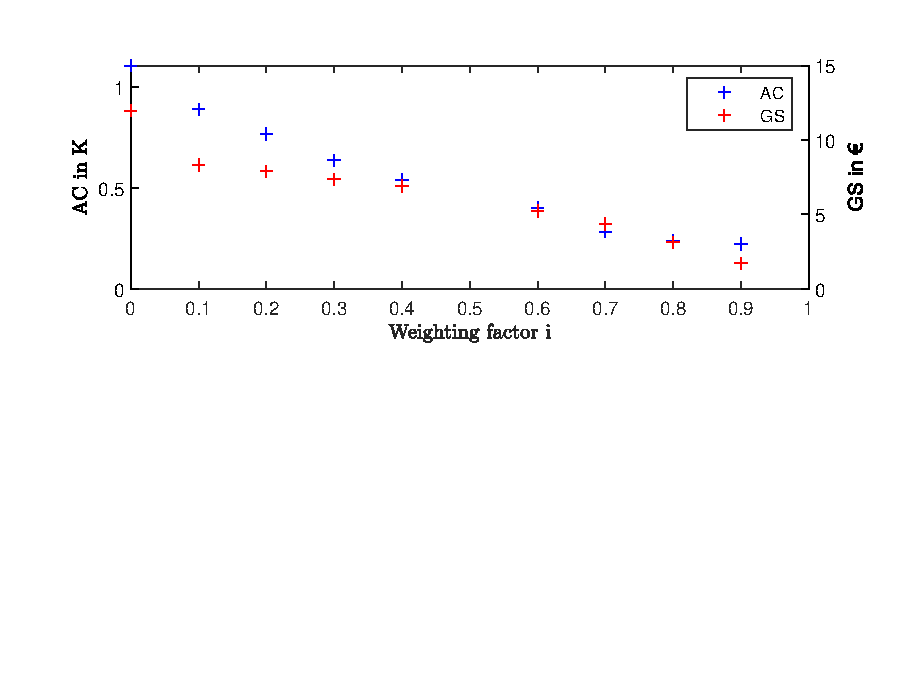
\includegraphics[width=15cm,height=8cm]{figure/AC_und_GS_12h.eps}
           \caption{AC and GS for N = 12h}
            \label{fig:AC_und_GS_12h}
    \end{figure}
    \begin{figure}[H]
            \centering
            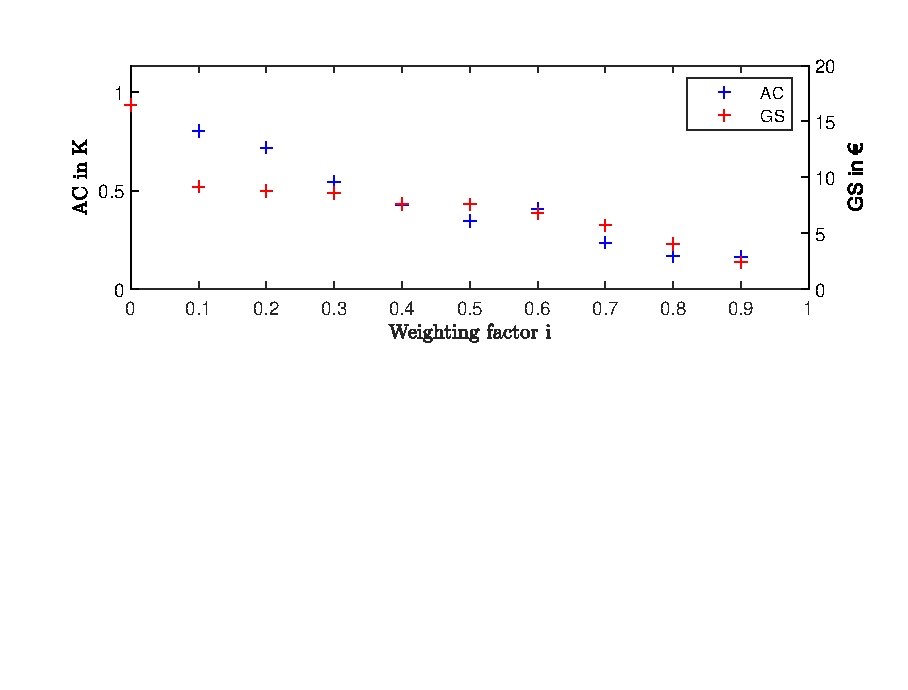
\includegraphics[width=15cm,height=8cm]{figure/AC_und_GS_18h.eps}
           \caption{AC and GS for N = 18h}
            \label{fig:AC_und_GS_18h}
    \end{figure}
     \begin{figure}[H]
            \centering
            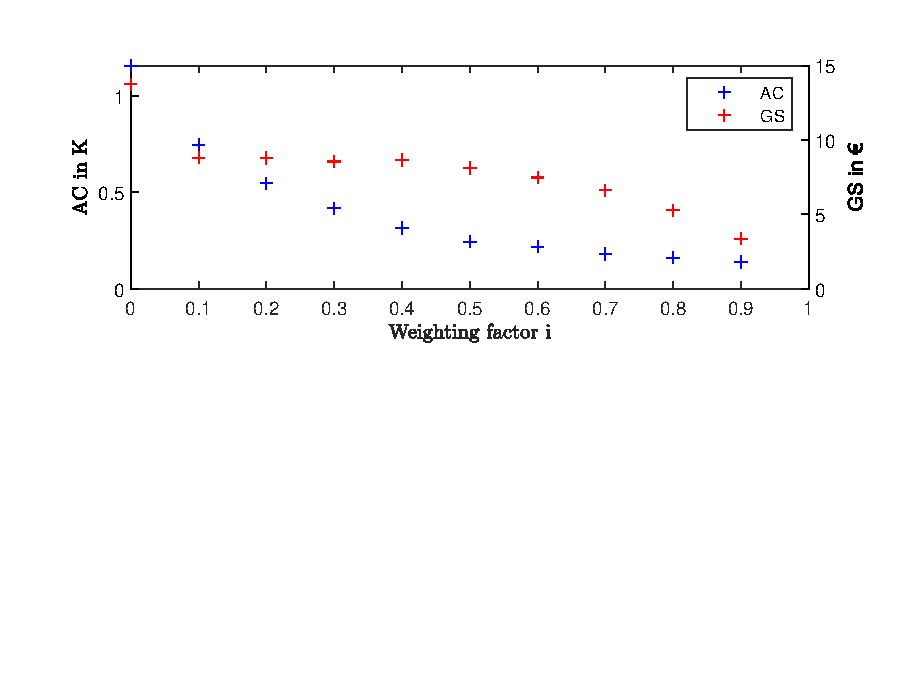
\includegraphics[width=15cm,height=8cm]{figure/AC_und_GS_30h.eps}
           \caption{AC and GS for N = 30h}
            \label{fig:AC_und_GS_30h}
    \end{figure}  		



\dots